\documentclass[aps,prl,reprint,10pt,amsmath,amssymb,superscriptaddress,a4paper]{revtex4-2}
\usepackage{xurl} % handle line breaks in long URL strings gracefully
\usepackage[utf8]{inputenc} % dding UNICODE support
\usepackage{indentfirst} % Indentation always (personal preference)
\usepackage[colorlinks=true,linkcolor=black,anchorcolor=black,citecolor=black,filecolor=black,menucolor=black,runcolor=black,urlcolor=black]{hyperref} % Hyper link for everything
\usepackage{graphicx} % Graphics package
\usepackage{dcolumn} % Double column package
\usepackage{amsmath, amsfonts, amsthm, physics} % Maths packages
\usepackage[margin=1cm]{geometry} % Sets 2cm margins
\usepackage{datetime} % Package for automatic date & time
\usepackage{enumerate} % Enumeration Package
\usepackage{listings} % To list code in your lab report
\usepackage{appendix} % This one kinda explains itself
\usepackage{float} % So the figures will behave
\usepackage{natbib}
\usepackage{tikz}

\begin{document}
\title{Coupled Pendula Lab Report}
\author{J. Liang (z5261830)}
\affiliation{Cohort B - Mon 9-12 class}
\affiliation{Word count: 2071 words}
\date{\currenttime~\today}
\begin{abstract}
    This report presents the theory, experimental observation and interpretations of the behaviour of coupled pendula.
\end{abstract}

\maketitle
\section{INTRODUCTION}
The behaviour of harmonic oscillators has been a long time interest for mathematicians and physicists. In this lab, I am going to present my observation and interpretations of the two normal modes and one of their linear combination mode (beat mode) of such a system with experimental data.
\par\noindent\rule{\linewidth}{0.4pt}

\section{AIM}
In this lab, the aim is to use the obtained data from the inphase oscillation, out of phase oscillation, and the beat mode, to quantitatively characterise the behaviours of coupled pendula system. Hence forward, establish a connection between this coupled system and its predecessor (a simple uncoupled pendulum) and its successor (many pendula all coupled together).
\par\noindent\rule{\linewidth}{0.4pt}

\section{Theory}
In this section, I am going to briefly discuss the derivations for three different modes for the coupled pendula and the notations I use.

\subsection{Assumptions}
First, it is important for the readers to know the assumption I have established. Note that those assumptions are in place to restrict this experiment in the scope of undergraduate physics.
\begin{enumerate}[I.]
    \item \textit{Small angle approximation} is used in the theoretical calculations of the equation of motions of the doubled pendula. \label{Assumption 1}
    \item The spring is in its equilibrium when the coupled pendula system is in its lowest energy state. In other words, the spring is not extended nor compressed when the pendula are not moving. \label{Assumption 2}
    \item The pendula are identical. \label{Assumption 3}
    \item The spring is equidistance from the top of both of the pendula. In other words, the spring is parallel to the ground. \label{Assumption 4} 
\end{enumerate}

\subsection{Derivations}
For the following section please refer to \textit{figure \ref{fig 1}} below for the variables that I did not specifically mentioned.
\begin{figure}[H]
    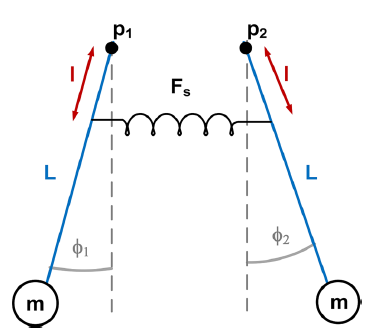
\includegraphics[width = 9 cm]{images/coupledpendula set up.png}
    \caption{The set up of the coupled pendula system.\citep{lab_note} \label{fig 1}}
\end{figure}
\begin{tikzpicture}
    \draw [thick,dash dot] (0,0) -- (9,0);
\end{tikzpicture}

\subsubsection{First Normal Mode}
The first normal mode of the coupled pendula system, is also known to be the in-phase oscillation mode. Is said to be when the two pendula are oscillating with the identical amplitude and frequency with no phase difference (\citeauthor{Taylor}, 2005, p. 423).

Note that in this mode, the spring is not being compressed nor extended. Therefore the spring have no contribution to the motion of the pendula. These two pendula will now have the same equation of motion which is identical to a single pendulum oscillating by itself. The equation of motion is
\begin{equation}
    \phi_1(t) = \phi_2(t) = \phi_{\text{max}} \cos (\omega_n t). \label{eq1}
\end{equation}
Where $\phi_{\text{max}}$ denotes the maximum amplitude of the pendula (note that both pendula have the same maximum amplitude), and $\omega_n$ denotes the natural \textbf{\emph{angular frequency}} of the system which is simply
\begin{equation}
    \omega_n = \sqrt{\frac{g}{L}}. \label{eq2}
\end{equation}

Note that the uncertainty of $\omega_n$ can be obtained by taking the Taylor expansion around zero, namely
\begin{equation}
    \Delta \omega_n = \sqrt{\left(\frac{\text{$\Delta $L} \sqrt{g}}{2 L^{3/2}}\right)^2+\left(\frac{\text{$\Delta $g}}{2 \sqrt{g L}}\right)^2}. \label{eq3}
\end{equation}

\begin{tikzpicture}
    \draw [thick,dash dot] (0,0) -- (9,0);
\end{tikzpicture}

\subsubsection{Second Normal Mode}
In the second normal mode, the pendula are oscillating with the same frequency and amplitude but they are perfectly out of phase (There is exactly $\pi$ radians difference between them). The equation of motions in this mode is now (\citeauthor{Taylor}, 2005, p. 425)
\begin{align}
    \phi_1(t) &= \phi_{\text{max}} \cos (\omega_o t)\\
    \phi_2(t) &= -\phi_{\text{max}} \cos (\omega_o t).
\end{align} 
With 
\begin{equation}
    \omega_o = \sqrt{\omega_n^2 + \frac{2kl^2}{mL^2}}, \label{eq6}
\end{equation}
and I obtained the uncertainty in similar fashion to the method used in obtaining eq. \ref{eq3}. Please refer to eq. \ref{eq7} in the \textbf{Long Equation} section for the uncertainty of $\omega_o$.

Unlike the first normal mode, the spring will contribute to the equation of motion in the second mode since it is being extended and compressed. Upon comparing eq. \ref{eq2} to eq. \ref{eq6}, it is obvious that 
$$\omega_o \ge \omega_n.$$
\begin{tikzpicture}
    \draw [thick,dash dot] (0,0) -- (9,0);
\end{tikzpicture}

\subsubsection{Beat Mode}
In this system, any oscillations between the two normal modes are a linear combination of the normal modes (they are also called the eigenstates which makes sense), and one interesting case is when the two combination contributes the same amount (imagine this as the mid point between two normal modes). And this is called the beat mode. The equation of motions governing this mode are 
\begin{align}
    \phi_1(t) &= \frac{\phi_{\text{max}}}{2} (\cos(\omega_o t) + \cos(\omega_n t))\\
    \phi_2(t) &= -\frac{\phi_{\text{max}}}{2} (\sin(\omega_o t) - \sin(\omega_n t)).
\end{align}
\begin{tikzpicture}
    \draw [thick,dash dot] (0,0) -- (9,0);
\end{tikzpicture}
\subsection{Coupling Factor}
The coupling factor, is a dimensionless constant that indicates how much influence the spring has on the system of the coupled pendula. And for the first normal mode it is almost trivial for one to realise that since the spring is not contributing to the system's movement. Therefore it would be rather silly to calculate the coupling factor. However, for the second normal mode and the beat mode the coupling factor can indeed offer us some insights on the behaviour of the system. 

The coupling factor for the second normal mode \cite{noauthor_coupled_nodate} and the normal mode are the same which is
\begin{equation}
    K_{\text{beat}} = K_{\text{out}} = \frac{\omega_o^2}{\omega_n^2+\omega_o^2}.
\end{equation}
The equation above immediately offered me the expectations that the slope and y-intercept from the data from trend (regression model) of the coupling factor should be identical for these two modes. Therefore, I have averaged out the coupling factor from the beat mode and the out of phase mode when calculating the trend of the experimental coupling factor.

And just for curiosity, let us observe what happens at the two extreme: very weak coupling and very strong coupling. Or in other words, when $l \to 0$ and $l \to \infty$. Notice that $\omega_o$ is proportional to $l$, so $\omega_o \to 0 \text{ as } l \to 0,$ and $\omega_o \to \infty \text{ as } l \to \infty$. It is not hard for us to see that the coupling factor for the extreme weak coupling case is 0 and for the extremely strong coupling case is 1, with all the possible coupling factors between 0 and 1.
\par\noindent\rule{\linewidth}{0.4pt}

\section{Method}\label{sec:method}
Firstly, the spring constant is measured using a number of weights. The spring is first place horizontally on the table to determined the equilibrium position (without it being affected by its own weight). Then, the changed of length are taken from each time a mass is added on the spring when it is hung vertically. The data are recorded, and to determined the spring's constant $k$. A linear regression model from SciPy\cite{2020SciPy-NMeth} is used (click \href{https://github.com/jojounderscorejo/CheatSheetRepo/blob/main/Otherthings/PHYS2113%20CP%20LAB/code/spring.ipynb}{\textbf{here}} for source code). Where the slope of the regression model is said to be the spring constant with the standard error of the regression model being the uncertainty in the spring's constant.

Two identical pendula are set up along side of each other. The spacing between the connecting rods of the pendula are adjusted to be the equilibrium position of the spring we are using. An angle to voltage transducer is used to record the amplitude as voltages and time for both of the pendula. The sampling interval is set to be 0.005 seconds. In this experiment, three different position for the spring's placement $l$ is used mainly 0.6, 0.4 and 0.2 metres.

The angle to voltage transducer is first calibrated by setting the zero voltage position at the stationary position (where $\phi_1 =\phi_2 = 0$).

\subsection{First Normal Mode}
For the first normal mode, also known as the in-phase oscillation mode. I brought two pendula to the same amplitude by slowing displacing the pendula from their equilibrium position with my fingers whilst observing the voltage reading at the computer. Then the pendula are let go at the same time. After releasing the pendula, I then start to record the data for a period of approximately 300 seconds.

\subsection{Second Normal Mode}
The second normal mode, or the out-out-phase oscillation mode is when the two pendula started at a position where $\phi_1(0) = - \phi_2(0).$ To achieve this, I used similar technique of to bring the pendula to their desired amplitude, this time with the exact opposite voltage reading on the computer for the two pendula. Then after releasing the pendula, the data are recorded for a period of approximately 300 seconds.

\subsection{Beat Mode}
To initiate the beat mode, one of the pendula must be at its maximum amplitude whilst the other is at it's equilibrium position. This is achieved by me placing one finger on the pendula that is supposed to be locked at its position to prevent it from moving whilst I bring the other pendula to the desired amplitude. Then I let go both of my fingers at the same time. Then the data is recorded for a period of 300 seconds.

The above set of three modes of measurements are carried out for three different spring distance $l$. 

The data collected is processed in python (click \href{https://github.com/jojounderscorejo/CheatSheetRepo/blob/main/Otherthings/PHYS2113%20CP%20LAB/code/CP%20data%20analysis-checkpoint.ipynb}{\textbf{here}} for source code) where a fast fourier transformed was performed using the NumPy FTT package \cite{harris2020array}, then the data are fitted with the a Lorentzian Curve using Python package LMFIT\cite{lmfit}. The code returns the data from the fit. Which I have taken the FWMH as the standard deviations (so the standard error would be half of the FWMH). 
\par\noindent\rule{\linewidth}{0.4pt}

\section{Results \& Analysis}
\subsection{The Spring constant}
This experiment would not have gone far without the me knowing the spring constant and its uncertainty. A graph of Length v.s. Mass on the spring is presented Figure 2. 
\begin{figure}[H]
    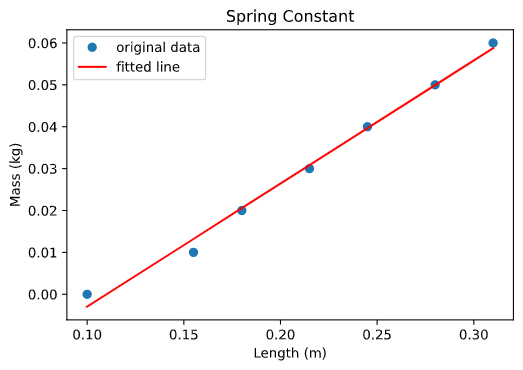
\includegraphics[width = 9 cm]{images/SpringConstant.png}
    \caption{A linear regression model for the spring constant. \label{fig 2}}
\end{figure}

Here, through the calculating the slope (times 9.8 ms$^{-2}$ to convert the mass to force). I have obtained the value of the spring constant to be 
\[
    k = 2.88 \pm 0.06 \text{ Nm}^{-1}.  
\]

\subsection{The Coupling Factor}
Now, through the method I have described in the \textbf{method} section, I have calculated the theoretical angular frequency for the three different coupling difference with the aid of Wolfram Mathematica\cite{math}, and the experimental value are calculated through my Python program. 

Inspecting Table \ref{table1}, I have notice there is an obvious systematic error. Where as the the theoretical value disagree with the experimental value by approximately 6\%. This disagreement is shown more with more pronunciation in figure \ref{fig3}. Where it clearly shows that the experimental value is clearly shifted upwards by approximately 6\%.

\begin{figure}[H]
    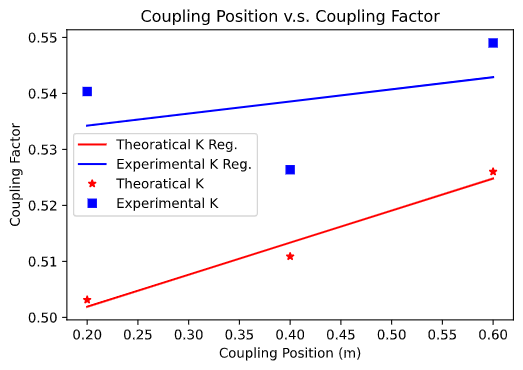
\includegraphics[width = 9 cm]{images/couplingfactor.png}
    \caption{A linear regression model for the spring constant. \label{fig3}}
\end{figure}
\par\noindent\rule{\linewidth}{0.4pt}

\section{DISCUSSION}
The uncertainty I have obtained does not offer me a satisfactory explanation of what is causing this deviation.

Thus, I shall now purpose a few scenarios that might have caused this systematic shift in the coupling factor;
\begin{enumerate}[Sc. I)]
    \item The mass of the rod was ignored in the theoretical calculation.
    \item The Pendula are not perfectly out of sync for the both of the normal modes.
    \item The pendula are not oscillating in the same plane.
\end{enumerate} 

Now, let us inspect the impact Sc. I has on this discrepancy. From equation \eqref{eq6}. We can determine the impact of the mass has on our system. By simply doing some trial calculation by substituting different $m$ in the theoretical calculation for $\omega_o$. I was only able to get a 6\% deviation for $\omega_o$ with 300\% of the original mass. Which clearly suggested to me that the mass of the rod has little to none effect on this double pendula system. 

Hence, Scenario I is deemed to in-sufficient to explain the deviation in our data. 

For the discussion regarding to Sc. II, I shall present you with the frequency domain graph for one of the oscillation.
\begin{widetext}

\begin{figure}[H]
    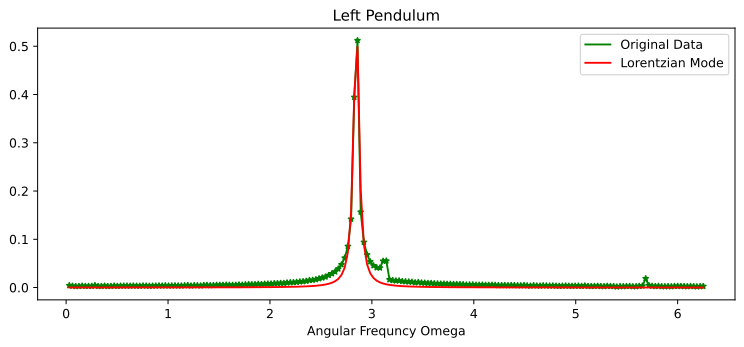
\includegraphics[width = 18 cm]{images/LM1.png}
    \caption{Frequency domain for the first normal mode for 0.6 m spring position. \label{fig4}}
\end{figure}

\begin{figure}[H]
    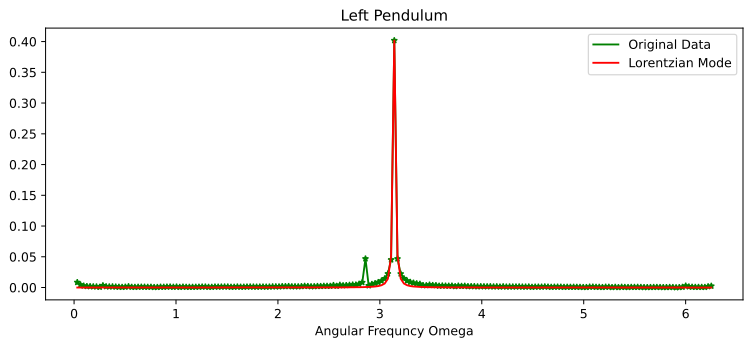
\includegraphics[width = 18 cm]{images/LM2.png}
    \caption{Frequency domain for the second normal mode for 0.6 m spring position. \label{fig5}}
\end{figure}
\end{widetext}

Upon inspecting Figure \ref{fig4} and Figure \ref{fig5}, it is obvious there indeed is a small peak presenting in the this frequency domain graph. From the theoretical calculation, it is clear that for both of the first and second normal mode. There should only be only one angular frequency that governs the equation of motion.

Figure \ref{fig4} and Figure \ref{fig5} are suggesting to me that there exists a consistent discrepancy for the initial value for both of these cases (i.e. I have not let go my hands simultaneously where one pendulum is a bit ``ahead'' of the other). 

However, the impact of this discrepancy between the assumption and the experimental condition is yet to be determined by me.
\par\noindent\rule{\linewidth}{0.4pt}

\section{Conclusion}
Based on the data on I have obtained, the experiment cannot be used to conclude or characterise the behaviour of the coupled pendula due to the large discrepancy between the experiment value and the theoretical calculations. However, if possible. Further measurements can be obtained in the lab and improvement can be made in regards to the measurement methods and therefore more meaningful ideas and conclusions can be extracted.








\newpage
\bibliographystyle{agsm}
\bibliography{cp.bib}
%%%%%%%%%%%%%%%%%%%%%%%%%%%%%%%%%%%%%%%%%%%%%%%%%
\onecolumngrid
\newpage
\appendix
\section{Appendix}
\section{Long Equations}\label{LE}
\begin{equation}
    \begin{split}
        \Delta \omega_o = \Biggl\{\frac{\text{$\Delta $l}^2 k^2 l^2}{L^4 m^2 \left(\frac{g}{L}+\frac{k l^2}{L^2 m}\right)}+\frac{\text{$\Delta $m}^2 k^2 l^4}{4 L^4 m^4 \left(\frac{g}{L}+\frac{k l^2}{L^2 m}\right)}&+\frac{\text{$\Delta $k}^2 l^4}{4 L^4 m^2 \left(\frac{g}{L}+\frac{k l^2}{L^2 m}\right)}+\\
        &\frac{\text{$\Delta $g}^2}{4 L^2 \left(\frac{g}{L}+\frac{k l^2}{L^2 m}\right)}+\frac{\text{$\Delta $L}^2 \left(-\frac{g}{L^2}-\frac{2 k l^2}{L^3 m}\right)^2}{4 \left(\frac{g}{L}+\frac{k l^2}{L^2 m}\right)}\Biggr\}^{1/2} \label{eq7}
    \end{split}
\end{equation}
\subsection{Experiment Data and Source Codes}
For the experiment data and the source code please visit this \href{https://github.com/jojounderscorejo/CheatSheetRepo/tree/main/Otherthings/PHYS2113%20CP%20LAB}{\textbf{link}}.

\section{Tables}
\begin{table}[H]
\centering
\caption{Theoretical v.s Experimental Values}
\begin{tabular}{|l|l|l|l|l|} \hline
\begin{tabular}[c]{@{}l@{}}Coupling length \\l (m)\\\end{tabular} & \begin{tabular}[c]{@{}l@{}}Theoretical \\Out of Phase \\Ag. Freq.\\(rad/s)\end{tabular} & \begin{tabular}[c]{@{}l@{}}Experimental\\Out of Phase \\Ag. Freq.\\(rad/s)\end{tabular} & \begin{tabular}[c]{@{}l@{}}Theoretical Beat Mode Ag. Freq. \\(rad/s)\end{tabular} & \begin{tabular}[c]{@{}l@{}}Experimental Out of Phase Ag. Freq\\(rad/s)\end{tabular} \\ \hline
0.2 & $3.20 \pm 0.10$ & $3.09 \pm 0.3$ & $\omega_n = 3.18 \pm 0.10 \;\&\; \omega_p = 3.20 \pm 0.10$ & N/A \\ \hline
0.4 & $3.25 \pm 0.10$ & $3.02\pm 0.01$ & $\omega_n = 3.18 \pm 0.10 \;\&\; \omega_p = 3.27 \pm 0.11$ & $\omega_n = 2.88 \pm 0.03\;\&\; \omega_p = 3.01\pm 0.02$ \\ \hline
0.6 & $3.35 \pm 0.11$ & $3.14\pm 0.1$ & $\omega_n = 3.18 \pm 0.10 \;\&\; \omega_p = 3.36 \pm 0.11$ & $\omega_n = 2.87 \pm 0.03\;\&\; \omega_p = 3.16\pm 0.03$ \\ \hline
\end{tabular}
\label{table1}
\end{table}

\end{document}